\section{Grammatiken und kontextfreie Sprachen}

% \datenote{18.11.16}
% Im folgenden Kapitel wechseln wir den Standpunkt von Spracherkennung auf \emph{Spracherzeugung}.
% Das Werkzeug sind hierbei sogenannte \emph{Phasenstrukturgrammatiken}, oder kurz, \emph{Grammatiken}.
% Bei Grammatiken gibt es neben dem Alphabet weitere Symbole, sogenannte \emph{Nichtterminalsymbole} oder \emph{Variablen}, und ein Regelsystem mit dem Wörter, die Nichtterminalsymbole enthalten, geändert werden können.
\begin{Def}
	Eine \emph{Grammatik} ist ein 4-Tupel $(\Sigma,N,P,S)$ mit folgenden Komponenten:
	\begin{itemize}
	\item $\Sigma$ ist ein Alphabet, dessen Elemente wir in diesem Kontext auch \emph{Terminalsymbole} nennen.
	\item $N$ ist eine endliche Menge, deren Elemente wir \emph{Nichtterminalsymbole} oder \emph{Variablen} nennen.
	\item $P\subseteq (N\cup\Sigma)^*N(N\cup\Sigma)^* \x (N\cup\Sigma)^*$ ist eine endliche Relation, 
	deren Elemente wir \emph{Regeln} oder \emph{Produktionen} nennen.
	\item $S\in N$ ist ein Nichtterminalsymbol, das wir \emph{Startsymbol} nennen.
	\qedhere
	\end{itemize}
\end{Def}

\begin{Bsp}\label{bsp:3.sameNumber}
  $\mathcal{G} = (\Sigma, N, P, S)$ mit\footnote{$P$ ist eine "`normale"' binäre Relation, 
  doch wir verwenden statt "`$(x,y)\in P$"' meist "`$x\-> y$"', also einen Pfeil und Infix-Notation, um die Lesbarkeit zu erhöhen.}
	\begin{align*}
		\Sigma &= \{ 0, 1 \}\\
		N &= \{S\}\\
		P &= \begin{aligned}[t]
      \{ S & \to 1S0S \\
        S & \to 0S1S \\
        S & \to \Eps
      \}
        \end{aligned}
      \qedhere
	\end{align*}
\end{Bsp}
% 
%   $G$ erzeugt geklammerte arithmetische Ausdrücke über der Konstante $\mathtt{a}$, wie zum Beispiel das Wort $\mathtt{(a*(a+a))}$.
%   Eine Grammatik erzeugt Wörter durch \emph{Ableitungen}, die wir im Folgenden definieren.
%   
\begin{Def}[Ableitungsrelation, Ableitung, Sprache einer Grammatik]
  Sei $\mathcal{G} =(\Sigma,N,P,S)$ eine Grammatik.
	Die \emph{Ableitungsrelation}\footnote{Analog zur Relation $P$ verwenden wir auch für die Ableitungsrelation wieder Infix-Notation, also $\alpha\vdash\beta$ statt $(\alpha,\beta)\in\;\vdash$.}
	zu $\mathcal{G}$ ist 
  \begin{displaymath}
    \cdot \vdash_\mathcal{G} \cdot \subseteq (N\cup\Sigma)^*\x(N\cup\Sigma)^*
  \end{displaymath}
  mit \ \ $\alpha \vdash_\mathcal{G} \beta$\ \  gdw\ \  $\alpha = \gamma_1\alpha'\gamma_2$,\ \  $\beta = \gamma_1\beta'\gamma_2$\ \  und \ \ $\alpha' \to \beta' \in P$

  Eine Folge $\alpha = \alpha_0,\ldots,\alpha_n = \beta$ heißt \emph{Ableitung von $\beta$ aus $\alpha$ in $n$ Schritten}, geschrieben $\alpha \stackrel{n}{\vdash}_\mathcal{G} \beta$, gdw $\alpha_i \vdash_\mathcal{G} \alpha_{i+1}$ für $0 \le i < n$.
  Jedes solche $\alpha_i$ heißt \emph{Satzform von $\mathcal{G}$}.

  Die \emph{Ableitung von $\beta$ aus $\alpha$}, geschrieben $\alpha \stackrel{*}{\vdash}_\mathcal{G} \beta$, existiert gdw ein $n \in \N$ existiert, sodass $\alpha \stackrel{n}{\vdash}_\mathcal{G} \beta$.
  Damit ist "`$\stackrel{*}{\vdash}_\mathcal{G}$"' die reflexive, transitive Hülle von "`$\vdash_\mathcal{G}$"'.

  Ein Wort $w\in\Sigma^*$ wird von $\mathcal{G}$ \emph{erzeugt}, wenn $S \stackrel{*}{\vdash}_{\mathcal{G}} w$ gilt.
	Die von $\mathcal{G}$ \emph{erzeugte Sprache} ist definiert als:
	\[ L(\mathcal{G}) = \{w\in\Sigma^* \mid S \stackrel{*}{\vdash}_{\mathcal{G}} w \}  \]
	
	Wir nennen zwei Grammatiken \emph{äquivalent}, wenn sie die gleiche Sprache erzeugen.
\end{Def}





\begin{Bsp}Wir betrachten nochmal die Grammatik aus \autoref{bsp:3.sameNumber}.\datenote{28.11.18}
Es gilt: $1001\in L(\mathcal{G})$.
$$ S 
\vdash_\mathcal{G} 1S0S
\vdash_\mathcal{G} 10S
\vdash_\mathcal{G} 100S1S
\vdash_\mathcal{G} 100S1
\vdash_\mathcal{G} 1001
$$
% \datenote{22.11.17}
Außerdem gilt: $L(\mathcal{G})$ ist die Sprache der Wörter über $\{0,1\}$, die gleich viele Nullen wie Einsen haben:
  \begin{displaymath}
    L = \{ w \in \Sigma^* \mid \#_0(w) = \#_1(w)\}
  \end{displaymath}
  Die Funktion $\#_a(w)$ berechnet hierbei die Anzahl der Vorkommen von $a \in \{0, 1\}$ in $w$.

  Dass $L(\mathcal{G}) \subseteq L$, lässt sich via Induktion über die Länge der Ableitung von $S \stackrel{*}{\vdash}_\mathcal{G} w$ zeigen.
  Der Beweis wird als Übung dem Leser überlassen.

  Wir zeigen $L \subseteq L(\mathcal{G})$.
  Dazu zeigen wir "`Wenn $w \in L$, dann $w \in L(\mathcal{G})$"' via Induktion über die Länge von $w$.
  Hierzu definieren wir noch die Hilfsfunktion $d : \Sigma^* \to \N$:
  \begin{align*}
    d(\Eps) &= 0 \\
    d(1w) &= d(w) + 1 \\
    d(0w) &= d(w) - 1
  \end{align*}
  Per Induktion über $|w|$ mit $w \in \Sigma^*$ lässt sich leicht zeigen, dass $L = \{w \in \Sigma^* \mid d(w) = 0\}$ und $d(v \cdot w) = d(v) + d(w)$.
  
Wir zeigen nun via Induktion über $n$ die folgende Eigenschaft:
$$\forall n' \leq n: \forall w \in \Sigma^*: \text{ falls } |w| = n' \text{ und } w \in L, \text{ dann } w \in L(\mathcal{G})$$

\begin{description}[font=\normalfont]
\item[I.A.:] $n = 0$: $w = \Eps$. Es gilt $\Eps \in L$, da $\#_0(\Eps) = \#_1(\Eps) = 0$.
% \item[IV] $\forall n' < n: \forall w' \in \Sigma^*: falls |w| = n' \text{ und } w \in L \text{ dann } w \in L(\mathcal{G})$
\item[I.S.:] $n \rightsquigarrow n+1$: $|w| = n > 1$, $w = aw'$, $a \in \{0,1\}$.
  Beachte: $|w|$ ist gerade für alle $w \in L$.

  Betrachte $a = 0$ (der Fall für $a = 1$ funktioniert analog).

  Da $0 = d(w) = d(0w') = d(w') - 1$, ist $d(w') = 1$.
  
  \medskip

  Wir zeigen zunächst, dass wir $w'$ in $w_11w_2$ mit $d(w_1) = 0$ und $d(w_2) = 0$ zerlegen können:
%   \begin{itemize}
%   \item[] 

    Sei $w' = a_1 \ldots a_n$.
    Betrachte die Folge $d_0,\ldots,d_n$ mit $d_0 = 0$ und $d_i = d(a_1\ldots a_i)$ für $1 \le i \leq n$.
    Wähle $0 \le i < n$ maximal, sodass für alle $0 \le j \le i$ gilt: $d_j < 1$.%
    \footnote{Wir wissen, dass $i < n$, da $d_n = d(w') = 1$.}

    Da $i$ maximal ist, folgt $d_{i+1} \ge 1$.
    Da $d_{j+1} - d_j \le 1$ für alle $0 \le j \le i$, folgt $d_{i+1} - d_i \le 1$ und damit auch $d_i = 0$, $d_{i+1} = 1$ und $a_{i+1} = 1$.
    Setze $w_1 = a_1\ldots a_{i}$.

    Es gilt also $w' = a_1\ldots a_{i}a_{i+1}w_2 = w_1w_2$ mit $d(w_1) = 0$.

    Da $d(v \cdot w) = d(v) + d(w)$ und $d(w') = d(w_11w_2) = 1$, folgt $d(w_2) = 0$.
%   \end{itemize}
  \bigskip
  \goodbreak

  Da $|w_1| < n$ und $|w_2| < n$, folgt nach I.V., dass $S \stackrel{*}{\vdash}_{\mathcal{G}} w_1$ und $S \stackrel{*}{\vdash}_{\mathcal{G}} w_2$.

  Es folgt mit den Regeln $S \vdash_{\mathcal{G}} 0S1S \stackrel{*}{\vdash}_{\mathcal{G}} 0w_11S \stackrel{*}{\vdash}_{\mathcal{G}} 0w_11w_2$.
  \qedhere
\end{description}
\end{Bsp}

\begin{Bsp}\label{bsp:3.anbncn}
	$\mathcal{G}=(\Sigma,N,P,S)$ mit
	\begin{align*}
		\Sigma &= \{a,b,c\}\\
		N &= \{S,B,C\}\\
		P &= 
		\begin{aligned}[t]
			 \{ &S \-> aSBC,\ S\->aBC,\ CB\-> BC,\ aB\-> ab,
			bB\-> bb, bC\-> bc, cC\-> cc \}
		\end{aligned}
% 		L(\mathcal{G}) &=  \{ a^nb^nc^n \mid n\geq 1 \}\\
% 		S &\=> aBC \=> abC \=> abc \qquad S\=>a\emph{S}BC \=> aa\emph{S}BCBC\\
% 		S &\=> aSBC \xRightarrow{n-2} n \=> a^{n-1}S(BC)^{n-1} \=> a^n(BC)^n = a^nBCBC \dots \=> a^nBBCCBC\\
% 		&\=> a^nB^nC^n \xRightarrow* a^nb^nc^n
	\end{align*}
Es gilt z.B. $aaabbbccc\in L(\mathcal{G})$.

Außerdem gilt $L(\mathcal{G}) =  \{ a^nb^nc^n \mid n\geq 1 \}$. (Ohne Beweis)
\end{Bsp}

\bigskip

Die Chomsky-Hierarchie teilt die Grammatiken in vier Typen unterschiedlicher Mächtigkeit ein.
\begin{Def}[Chomsky-Hierarchie]\
	\begin{itemize}
	\item Jede Grammatik ist eine \emph{Typ-0-Grammatik}.
	\item Eine Grammatik ist \emph{Typ-1} oder
          \emph{kontextsensitiv}, falls alle Regeln expansiv sind,
          d.h., für alle Regeln $\alpha\->\beta\in P$ ist
          $|\alpha|\leq |\beta|$. Ausnahme: falls $S$ nicht in einer
          rechten Regelseite auftritt, dann ist $S\->\Eps$ erlaubt. 
	\item Eine Grammatik heißt \emph{Typ-2} oder \emph{kontextfrei}, falls alle Regeln die Form $A\->\alpha$ mit $A\in N$ und $\alpha\in(N\cup\Sigma)^*$ haben.
	\item Eine Grammatik heißt \emph{Typ-3} oder \emph{regulär}, falls alle Regeln die folgende Form haben:
	\begin{alignat*}{2}
		&A\->w &\quad w&\in\Sigma^*\\
		\text{oder}\quad &A\->aB& a&\in\Sigma,\ B\in N
	\end{alignat*}
	\end{itemize}
	Eine Sprache heißt Typ-$i$-Sprache, falls es eine Typ-$i$-Grammatik für sie gibt.
\end{Def}

\begin{Beobachtung}\label{beob:3.ChomskyHierarchie}
	Jede Typ-$(i+1)$-Sprache ist auch eine Typ-$i$-Sprache.
\end{Beobachtung}
\begin{itemize}
 \item Jede Typ-3-Grammatik ist eine Typ-2-Grammatik.
 \item Wir werden im folgenden Unterkapitel zeigen, dass jede Typ-2-Grammatik in eine äquivalente $\Eps$-freie\footnote{Auf keiner rechten Seite steht $\Eps$; Ausnahme: Startsymbol $S$; vgl. Elimination von $\Eps$-Produktionen.} Typ-2-Grammatik transformiert werden kann.
 Diese erfüllt dann auch alle Bedingungen einer Typ-1-Grammatik.
 \item Jede Typ-1-Grammatik ist auch eine Typ-0-Grammatik.
\end{itemize}

Im Lauf der Vorlesung werden wir die folgende Aussage zeigen:\\
Sei $CHi$ die Menge der Typ-$i$ Sprachen; dann gilt: 
$CH3 \subsetneq CH2 \subsetneq CH1 \subsetneq CH0$.




\subsection{Kontextfreie Sprachen}\datenote{30.11.2018}
Die Sprache aus \autoref{bsp:3.sameNumber} ist kontextfrei. Weitere Beispiele sind:

\begin{Bsp}\label{bsp:3.ArithExpr}
Arithmetische Ausdrücke ohne Klammern: 
$\mathcal{G}=(\{E\}, \{a, \mathnormal{+}, \mathnormal{*}\}, P, E)$ mit
\begin{displaymath}
 P = \{ E \->a \mid E+E \mid E*E\}.
 \footnote{Notation: Wenn wir mehrere Regeln mit gleicher linker Seite wie 
 z.B. "`$A \-> \alpha$"' und "`$A \-> \beta$"' haben, dann dürfen wir diese auch mit Hilfe eines senkrechten Striches als "`$A \-> \alpha\mid\beta$"' schreiben.}
 \qedhere
\end{displaymath}
\end{Bsp}

\begin{Bsp}
Arithmetische Ausdrücke mit Klammern: 
$\mathcal{G}=(\{E\}, \{a, \mathnormal{+}, \mathnormal{*}, \mathnormal{(}, \mathnormal{)}\}, P, E)$ mit
  \begin{displaymath}
    P = \{ E \->a \mid (E+E) \mid (E*E)\}.
  \qedhere
  \end{displaymath}
\end{Bsp}
% 
\newcommand{\boxedt}[1]{\tikz[baseline]{\node[shape=rectangle,draw=lightgray,fill=lightgray!50,inner sep=0pt] at (0,.64ex){\hspace{.3em}\texttt{\strut#1}\hspace{.3em}\strut};}}
% 
\begin{Bsp}
Syntax von Programmiersprachen. 
Wir zeigen hier nur exemplarisch Produktionen für einige typische Bestandteile einer Programmiersprache.\footnote{
Sie finden am Ende der Java Language Specification \url{https://docs.oracle.com/javase/specs/} auf ca.\ 25 Seiten die kontextfreie Grammatik für diese Programmiersprache.
}
Wörter in spitzen Klammern sind hier Nichtterminalsymbole.
Terminalsymbole sind grau unterlegt.
	\begin{center}
		\begin{tabular}[t]{r@{ }l}
			<Stmt> \-> & <Var> \boxedt{=} <Exp>\\
			|\, & <Stmt>\,\boxedt{;}\,<Stmt>\\
			|\, & \boxedt{if}\,\boxedt{(}<Exp>\boxedt{)} <Stmt> \boxedt{else} <Stmt>\\
			|\, & \boxedt{while}\,\boxedt{(}<Exp>\boxedt{)} <Stmt>
		\qedhere
		\end{tabular}
	\end{center}
\end{Bsp}

% \begin{Bsp}
%  \item Palindrome über $\{a,b\}$
% 	\[ S\-> aSa \mid bSb \mid a \mid b \mid \Eps \]
% \end{Bsp}

%Abk.: \aclu{CFL}: \acs{CFL}\\
%\phantom{Abk.:} \aclu{CFG}: \acs{CFG}


Für den arithmetischen Ausdruck ohne Klammern $a+a$ gibt es in der Grammatik aus \autoref{bsp:3.ArithExpr} zwei verschiedene Ableitungen:
\begin{itemize}
 \item $E\vdash_\mathcal{G} E+E\vdash_\mathcal{G} a+E\vdash_\mathcal{G} a+a$
 \item $E\vdash_\mathcal{G} E+E\vdash_\mathcal{G} E+a\vdash_\mathcal{G} a+a$
\end{itemize}
Beide Ableitungen unterscheiden sich nur durch die Reihenfolge, in der Variablen ersetzt werden.
Die folgende Definition erlaubt es uns, beide Ableitungen durch das gleiche Objekt,
den sogenannten Ableitungsbaum, darzustellen.


\newcommand{\T}{\mathcal{T}}

\begin{Def}[name={[Ableitungsbaum]}] Sei $\mathcal{G} = (\Sigma, N, P, S)$ eine kontextfreie Grammatik.
  Wir definieren die Menge der \emph{in $A$ beginnenden Ableitungsbäume von $\mathcal{G}$}, $\operatorname{Abl}(A)$, für $A\in N$ als Menge von beschrifteten, geordneten Bäumen induktiv wie folgt:
  
  Falls $\pi = A \to w_0A_1w_1\ldots A_nw_n \in P$ mit $A_i \in N$, $w_0, w_i \in \Sigma^*$, $1 \le i \le n$ und $\T_i \in \operatorname{Abl}(A_i)$, dann ist
    \begin{center}
			\tikz[baseline=0cm]{\Tree [.$\pi$ $\T_1$ \edge[draw=none]; {$\dots$} $\T_n$ ]} $\in \operatorname{Abl}(A)$
    \end{center}
    Da es manchmal aufwendig ist, Bäume zu zeichnen, verwenden wir alternativ die folgende Notation: $\pi(\T_1, \ldots, \T_n)$

    Das \emph{abgeleitete Wort zu einem $\T \in \operatorname{Abl}(A)$}, $Y(\T)$\footnote{Wir verwenden $Y(\T)$, um an das englische Wort "`yield"' zu erinnern.}, ist definiert durch
    \begin{displaymath}
      Y\left(\tikz[baseline=-0.4cm]{\Tree [.$\pi$ $\T_1$ \edge[draw=none]; {$\dots$} $\T_n$ ]} \right) = w_0Y(\T_1)w_1\ldots Y(\T_n)w_n
    \end{displaymath}
    wobei $\pi = A \to w_0A_1w_1\ldots A_nw_n \in P$.
\end{Def}

\begin{Bemerkung}
Nach dieser Definition gibt es also insbesonere für jede Regel $\pi$ bei der nur Terminalsymbole auf der rechten Seite vorkommen einen Ableitungsbaum der die einelementige Knotenmenge $\{\pi\}$ und einer leeren Menge von Kanten hat.
\end{Bemerkung}



\begin{Bsp}\label{bsp:Ableitungsbaum} 
Für die Grammatik aus \autoref{bsp:3.ArithExpr} sind die folgenden drei Beispiele in $E$ beginnende Ableitungsbäume.

    \tikz[baseline=0cm]{\Tree [ .$E\to a$ ]}
    \hfill
    \tikz[baseline=0cm]{\Tree [ .$E\to E+E$ $E\to a$ [ .$E\to E*E$ $E\to a$ $E\to a$ ] ]}
    \hfill
    \tikz[baseline=0cm]{\Tree [ .$E\to E*E$ [ .$E\to E+E$ $E\to a$ $E\to a$ ] $E\to a$ ]}
\end{Bsp}

\begin{lemma}
  Sei $\mathcal{G} = (\Sigma, N, P, S)$ eine kontextfreie Grammatik.
  \begin{displaymath}
    w \in L(\mathcal{G})  \quad\text{ gdw }\quad \exists \;\T \in \operatorname{Abl}(S) \text{ mit } Y(\T) = w
    \qedhere
  \end{displaymath}
\end{lemma}
(Ohne Beweis.)

% \begin{proof}[$\Longrightarrow$]
%   Wir zeigen via vollständiger Induktion über die Länge der Ableitung $n$:
%   \begin{displaymath}
%    \forall n \in \N: \forall w \in \Sigma^*: \forall A \in N: A \stackrel{n}{\==>} w \text{ dann } \exists \T \in \operatorname{Abl}(\mathcal{G}, A) \text{ mit } Y(\T) = w
% \end{displaymath}
%    \begin{description}
%    \item[IA] $n=0$ (nichts zu tun, da $A \stackrel{n}{\==>} \Eps$ unmöglich)
%    \item[IS] Sei $n > 0$: $A \stackrel{n}{\==>}$ hat die Form
%      \begin{displaymath}
%        A {\==>} w_0A_1w_1\ldots A_nw_n \stackrel{n-1}{\==>} w
%      \end{displaymath}
%      Also ist $w = w_0v_1w_1\ldots v_nw_n$ mit $A_i \stackrel{n_i}{\==>} v_i$ für $1 \le i \le n$ und $n_i < n$.\footnote{Dieser Beweisschritt ist nicht ganz präzise\ldots die Ableitungen der $v_i$ sind nicht unbedingt Teil der gesamten Ableitung $A \stackrel{n}{\Longrightarrow} w$.
%      Man kann aber beweisen dass eine alternative Ableitung existieren muss, bei der dies der Fall ist.}
%    Nach IV ergibt sich
%    \begin{displaymath}
%      \exists \T_i \in \operatorname{Abl}(G, A_i) \text{ mit } Y(\T_i) = v_i
%    \end{displaymath}
%    Dann ist $\T = \pi(\T_1,\ldots, \T_n)$ mit $\pi = A \to w_0A_1w_1\ldots A_nw_n \in \operatorname{Abl}(\mathcal{G}, A)$ und $Y(\T) = w_0Y(\T_1)w_1\ldots Y(\T_n)w_n= w_0v_1w_1\ldots v_nw_n$.
%    \end{description}
% \end{proof}
% 
% \begin{proof}["`rechts nach links"']
%   Zu zeigen:
%   \begin{displaymath}
%     \forall n \in \N: \forall \T \in \operatorname{Abl}(\mathcal{G}, A): \text{falls } Y(\T) = w \text{ dann } A \stackrel{*}{\==>} w
%   \end{displaymath}
%   \begin{description}
%   \item[IS]
% \footnote{ Der Induktionsanfang ist bei Ableitungsbäumen ein Spezialfall des Induktionsschritts (Bäume ohne Kinder bzw.\ Regeln, die nur Terminale ableiten) und wird daher nicht gesondert aufgeführt }
%     Falls für $n \ge 0$
%     \begin{itemize}
%     \item  $\T = \pi(\T_1, \ldots, \T_n)$,
%     \item $\pi = w_0A_1w_1\ldots A_nw_n$,
%     \item $\T_i \in \operatorname{Abl}(\mathcal{G}, A_i)$,
%     \item $Y(\T) = w_0Y(\T_1)w_1\ldots Y(\T_n)w_n$
%     \end{itemize}
%     dann gilt nach IV:\footnote{Strengenommen müsste die Folgerung, die hier mit "`\ldots"' abgekürzt ist noch via Induktion über Ableitungen gezeigt werden} 
%     \begin{align*}
%       A &\==> w_0A_1\ldots A_nw_n \\
%         &\stackrel{*}{\==>} w_0Y(\T_1)\ldots A_nw_n \\
%         & \dots \\
%         & \stackrel{*}{\==>} w_0Y(\T_1)\ldots Y(\T_n)w_n \\
%         &= w
%     \end{align*}
%   \end{description}
%   
% \end{proof}

\begin{Def}[name={[Eindeutigkeit von \acs*{CFG} und \acs*{CFL}]}]\
	\begin{itemize}
% 	\item Sei CFG die Menge der kontextfreien Grammatiken.
  \item Eine Grammatik $\mathcal{G}$ heißt \emph{eindeutig}, falls es für jedes Wort $\in L(\mathcal{G})$ genau einen Ableitungsbaum gibt.
	\item Eine kontextfreie Sprache $L$ heißt \emph{eindeutig}, falls es eine eindeutige kontextfreie Grammatik gibt, die $L$ erzeugt.
	\qedhere
	\end{itemize}
\end{Def}
% \begin{Bsp}
% 	\begin{align*}
% 		L &= \{ a^ib^jc^k \mid i=j\text{ oder }j=k \}\\
% 		S &\-> AC \mid DB\\
% 		A &\-> aAb \mid \Eps & D &\->aD \mid \Eps\\
% 		C &\->cC \mid \Eps & B &\-> bBc \mid \Eps \quad[\text{für $L$ gibt es keine eindeutige \ac{CFG}}]
% 	\end{align*}
% 	Werte der Form $a^nb^nc^n$ haben zwei Ableitungen $\curvearrowright$ Grammatik ist nicht eindeutig.
% \end{Bsp}

Die Grammatik aus \autoref{bsp:3.ArithExpr} ist also nicht eindeutig, denn sowohl für den zweiten als auch für den dritten Ableitungsbaum aus \autoref{bsp:Ableitungsbaum} ist das abgeleitete Wort $a+a*a$.

Im Folgenden verwenden wir auch die Abkürzung \acsu{CFG} für "`kontextfreie Grammatik"' (engl.\ context-free grammar).



\subsection{Die Chomsky-Normalform für kontextfreie Sprachen}\label{sec:cnf}
% Notwendig für das Pumping Lemma kontextfreier Sprachen und für einen effizienten Algorithmus für das \nameref{satz:wortproblem}.
Wir lernen in diesem Unterkapitel eine spezielle Form von kontextfreien Grammatiken (Chomsky-Normalform) kennen, für die gilt:
\begin{itemize}
 \item Das Wortproblem ($w\in L(\mathcal{G})$?) lässt sich mit Hilfe eines einfachen Algorithmus entscheiden.
 \item Jede kontextfreie Grammatik lässt sich "`effizient"' in diese Normalform transformieren.
\end{itemize}

Wir stellen im Folgenden vier Transformationen (\textsc{Sep, Bin, Del, Unit}) 
vor und wollen dabei jeweils den Zeitaufwand und die Größe der resultierenden \ac{CFG} analysieren.

Dafür definieren wir die Größe einer Grammatik wie folgt.
\begin{displaymath}
  |\mathcal{G}| = \sum_{A \in N}\sum_{A \to \alpha \in P} |A\alpha|
\end{displaymath}
Die Größe ist also genau die Anzahl an Zeichen aus $\Sigma\cup N$, die man benötigt, um die Regeln der Grammatik aufzuschreiben.

\begin{Def}
  Eine \ac{CFG} heißt \emph{separiert}, wenn jede Regel eine der folgenden beiden Formen hat.
  \begin{alignat*}{3}
   A &\-> A_1\dots A_n && \quad \text{für } A\in N, A_i\in N,n\geq 0\\[1mm]
   A &\-> a && \quad \text{für } A\in N, a\in\Sigma
  \qedherefixalignat
  \end{alignat*}
\end{Def}

\begin{lemma}[\textsc{Sep}]
  Zu jeder \ac{CFG} gibt es eine äquivalente separierte \ac{CFG}.
\end{lemma}
\begin{proof}
  Sei $\mathcal{G} = (\Sigma, N, P, S)$ eine \ac{CFG}.
  Konstruiere $\mathcal{G}' = (\Sigma, N', P', S)$ mit
  \begin{itemize}
  \item $N' = N \overset.\cup \{Y_a \mid a \in \Sigma \}$\footnote{"`$\overset.\cup$"' steht für "`disjunkte Vereinigung"'}
  \item $P' = \{Y_a \to a \mid a \in \Sigma \} \cup \{A \to \beta[a \to Y_a] \mid A \to \beta \in P \}$.
  
    Die Schreibweise $\beta[a\to Y_a]$ bedeutet hier, dass alle $a \in \Sigma$, die in $\beta$ vorkommen, durch $Y_a$ ersetzt werden.
  \end{itemize}
  Offenbar gilt $L(\mathcal{G}) = L(\mathcal{G'})$ und $\mathcal{G}'$ ist separiert (ohne Beweis).
\end{proof}
\begin{Bemerkung}
\textsc{Sep} berechnet in $O(|\mathcal{G}|^2)$ eine Grammatik der Größe $O(|\mathcal{G}|)$.
\begin{itemize}
	\item Laufe für jedes Terminalsymbol einmal über alle Regeln.
	
	\item Für jedes neue Nichtterminalsymbol fügen wir eine Regel der Größe 2 hinzu.
	\qedhere
\end{itemize}
\end{Bemerkung}



\begin{lemma}[\textsc{Bin}]
  Zu jeder \ac{CFG} gibt es eine äquivalente \ac{CFG}, bei der für alle Regeln $A \to \alpha$ gilt, dass $|\alpha| \le 2$.
\end{lemma}
\begin{proof}
  Ersetze jede Regel der Form 
  \begin{displaymath}
    A \to X_1X_2\ldots X_n, \quad n\geq 3
  \end{displaymath}
  mit $X_i \in N \cup \Sigma$, $1 \le i \le n$,
  durch die Regeln 
  \begin{align*}
    A &\to X_1\langle  X_2\ldots X_n \rangle \\
    \langle  X_2\ldots X_n \rangle & \to X_2\langle  X_3\ldots X_n \rangle \\
    \vdots \\
    \langle  X_{n-1}X_n \rangle & \to X_{n-1}X_n
  \end{align*}
  Dabei sind  $\langle  X_2\ldots X_n \rangle$, \ldots, $\langle  X_{n-1}\ldots X_n \rangle$ neue Nichtterminalsymbole.
\end{proof}
\begin{Bemerkung}
\textsc{Bin} berechnet in $O(|\mathcal{G}|)$ eine Grammatik der Größe $O(|\mathcal{G}|)$.
\begin{itemize}
	\item Laufe einmal über alle Regeln.
	
	\item Für jede Regel der Größe $n+1$, $n\geq 3$ fügen wir höchstens $n-1$ neue Regeln der Größe 3 hinzu.
	\qedhere
\end{itemize}
\end{Bemerkung}


Wir definieren die Menge der Nichtterminalsymbole, aus denen das leere Wort abgeleitet werden kann, formal wie folgt:
\begin{Def}
  Sei $\mathcal{G} = (\Sigma, N, P, S)$ eine \ac{CFG}.
  Definiere die Menge $\operatorname{Nullable}(\mathcal{G}) \subseteq N$ als
  \begin{displaymath}
    \operatorname{Nullable}(\mathcal{G}) = \{ A \in N \mid A
    \stackrel{*}{\vdash}_\mathcal{G} \Eps \}
    \text{.} \qedhere
  \end{displaymath}
\end{Def}

\begin{Satz}\label{satz:3.nullable}\datenote{5.12.2018}
  Es gibt einen Algorithmus, der $\operatorname{Nullable}(\mathcal{G})$ in $O(|\mathcal{G}|^3)$ berechnet.
\end{Satz}
\begin{proof}
  Definiere $M_i$ als die Menge der Nichtterminalsymbole, aus denen sich
  $\Eps$ mit einem Ableitungsbaum der Höhe $< i$ ableiten lässt:\footnote{
  Im Folgenden ist mit $*$ bei $M_i^*$ und $M^*$ der Kleene-Stern gemeint.} 
  \begin{align*}
    M_0 &= \emptyset \\
    M_{i+1} &= M_i \cup \{ A \mid A \to \alpha \in P \text{ und }
              \alpha \in M_i^* \}
  \end{align*}
  Es gilt für alle $i \in \N$, dass $M_i \subseteq N$.
  Da $|N|$ endlich ist, existiert ein $m \in \N$, sodass
  \begin{displaymath}
    M_m = M_{m+1} = \bigcup_{i \in \N} M_i
  \end{displaymath}
  Wir können $\bigcup_{i \in \N} M_i$ mit dem folgenden Verfahren in $O(|\mathcal{G}|^3)$ berechnen.
  
  \begin{center}
  \begin{minipage}{7cm}
  \begin{lstlisting}[
  mathescape,
  columns=fullflexible,
  basicstyle=\fontfamily{lmvtt}\selectfont,
]
M = {}
done = $false$
while (not done):
    done = $true$
    M$_{old}$ = M
    foreach $A \to a \in P$:
         if ($ A \not \in M \wedge a \in M_{old}^*$):
             $M = M \cup \{A\}$
             done = $false$
return M
\end{lstlisting}
\end{minipage}
\end{center}

  Wir zeigen nun, dass $\operatorname{Nullable}(\mathcal{G}) = \bigcup_{i \in \N} M_i$.

  \medskip
  
  "`$\supseteq$"'\quad
  Wir zeigen via Induktion über die Höhe des Ableitungsbaums $i$, dass 
  $$\forall i \in \N: M_i \subseteq \operatorname{Nullable}(\mathcal{G})$$
  \begin{description}
  \item[IA] $i = 0$: $M_0 = \emptyset \subseteq \operatorname{Nullable}(\mathcal{G})$
  \item[IS] $i \rightsquigarrow i+1$

    Wenn $A \in M_{i+1}$, dann
    \begin{itemize}
    \item gilt entweder
      $A \in M_i \subseteq \operatorname{Nullable}(\mathcal{G})$ nach
      IV oder
    \item 
      es existiert $A \to A_1\ldots A_n \in P$ mit $A_j \in M_i$ für
      $1 \le j \le n$.
      Nach IV existieren Ableitungen
      \begin{displaymath}
        A_j \stackrel{*}{\vdash}\mathcal{G} \Eps
      \end{displaymath}
      sodass auch eine Ableitung von $A$ nach $\Eps$ existiert:
      \begin{displaymath}
        A  \vdash_\mathcal{G} A_1 \ldots A_n \stackrel{*}{\vdash}\mathcal{G} \underbrace{\Eps \ldots \Eps}_{n \text{ Mal}} = \Eps
      \end{displaymath}
      Also gilt $A \in \operatorname{Nullable}(\mathcal{G})$.
    \end{itemize}
  \end{description}

  \medskip
  
  "`$\subseteq$"'\quad
  Wenn $A \in \operatorname{Nullable}(\mathcal{G})$, dann existiert $m
  \in \N$, sodass $A \stackrel{*}{\vdash}\mathcal{G} \Eps$ mit einem
  Ableitungsbaum der Höhe $m$.
  Wir zeigen via Induktion über $m$, dass $A \in M_{m+1} \subseteq \bigcup_{i \in \N} M_i$.
  \begin{description}
  \item[IA] $m = 1$. Die Ableitung ist $A \vdash_\mathcal{G} \Eps$, sodass $A\in M_1$.
  \item[IS] $m > 1$.
    Die Wurzel des Ableitungsbaum muss mit $A \to A_1\ldots A_n$ ($n>0$)
    beschriftet sein und die Kinder sind jeweils Ableitungsbäume für
    $\Eps$ in  $Abl(A_i)$ der Höhe $m_i \le m-1$, wobei $1 \le i \le n$.
    
    Es gilt nun nach IV, dass $A_i \in M_{m_i} \subseteq M_{m-1}$.
    Somit ist $A_i \in M_{m-1}$ und damit, nach Definition, $A \in M_m$.
    \qedhere
  \end{description}
\end{proof}

\begin{Korollar}
  Man kann zu einer \ac{CFG} $\mathcal{G}$ berechnen, ob $\Eps \in L(\mathcal{G})$.
\end{Korollar}
\begin{proof}
  Prüfe, ob $S \in \operatorname{Nullable}(\mathcal{G})$.
\end{proof}
\begin{lemma}[\textsc{Del}]
  Zu jeder \ac{CFG} $\mathcal{G}=(\Sigma, N, P, S)$ gibt es eine äquivalente \ac{CFG} $\mathcal{G'} =(\Sigma, N', P', S')$, bei der die einzige $\Eps$-Regel $S' \to \Eps$ ist (falls $\Eps \in L(\mathcal{G})$) und bei der $S'$ auf keiner rechten Seite einer Regel vorkommt.
\end{lemma}
\begin{proof}
  \hfill
  \begin{enumerate}
  \item Erweitere $\mathcal{G}$ um ein neues Startsymbol $S' \notin N$ mit $S' \to S$ als neue Regel.
    Dieser Schritt stellt sicher, dass $S'$ auf keiner rechten Regelseite vorkommt.
  \item Wende erst \textsc{Sep}, dann \textsc{Bin} an.
    Nun hat jede rechte Regelseite die Form $a \in \Sigma$ oder $\Eps$ oder $A$ oder $BC$.
  \item Für alle Regeln $A \to BC \in P$:
    \begin{itemize}
    \item Falls $B \in \operatorname{Nullable}(\mathcal{G})$ füge $A \to C$ hinzu.
    \item Falls $C \in \operatorname{Nullable}(\mathcal{G})$ füge $A \to B$ hinzu.
    \end{itemize}
  \item Falls $S \in \operatorname{Nullable}(\mathcal{G})$, füge $S' \to \Eps$ hinzu
  \item Entferne alle Regeln $A \to \Eps$ für $A \neq S'$.
  \qedhere
  \end{enumerate}
\end{proof}
\begin{Bemerkung}
\textsc{Del} kann in $O(|\mathcal{G}|^3)$ berechnet werden und die Größe der resultierenden Grammatik ist $O(|\mathcal{G}|)$.
\begin{itemize}
	\item Die höchsten Kosten entstehen beim Berechnen von Nullable.
	
	\item In Schritt 3 verdoppelt sich die Anzahl der Regeln höchstens.
	\qedhere
\end{itemize}
\end{Bemerkung}

\begin{Def}
  Sei $\mathcal{G} = (\Sigma, N, P, S)$ eine Grammatik.
  Eine \emph{Kettenregel} von $\mathcal{G}$ ist eine Regel in $P$ der Form $A \to B$, wobei $A,B \in N$.
\end{Def}

\datenote{7.12.2018}
\begin{lemma}[\textsc{Unit}]
Es gibt einen Algorithmus der für eine \ac{CFG} $\mathcal{G}$ in $O(|\mathcal{G}|^3)$ eien äquivalente \ac{CFG} $\mathcal{G}'$ ohne Kettenregeln mit $|\mathcal{G}'|\in O(|\mathcal{G}|^2)$ berechnet.
%   Zu jeder \ac{CFG} $\mathcal{G} = (\Sigma, N, P, S)$ gibt es eine äquivalente \ac{CFG} $\mathcal{G}' = (N, \Sigma, P', S)$ ohne Kettenregeln.
\end{lemma}
\begin{proof} (Beweisskizze)
	\begin{itemize}
	\item Zur Äquivalenz:
	
	Wir zeigen dass jeden Schritt der die \ac{CFG} ändert eine äquivalente \ac{CFG} liefert.
	Dazu zeigen wir dass es für jedes Wort dass in der alten \ac{CFG} abgeleitet werden konnte auch in der neuen \ac{CFG} abgeleitet werden kann und umgekehrt.
	Für Schritt~\ref{alg:unit-step-chain} können wir -- es macht den Beweis etwas einfacher -- zeigen dass Äquivalenz sogar für jede Iteration der mittleren for-Schleife gilt.
	
	\item Zur Kettenregelfreiheit:
	
	In Schritt~\ref{alg:unit-step-DelCycle} wird mindestens ein Kettenregelzykel entfernt und da eine Grammatik nur endlich viele Regeln hat wird nach spätestens $|\mathcal{G}|$ Anwendungen von Schritt~\ref{alg:unit-step-DelCycle} der Schritt~\ref{alg:unit-step-dag}, in dem alle Zykeln entfernt sind, erreicht.
	
	In der mittleren for-Schleife von Schritt~\ref{alg:unit-step-chain} gilt aufgrund der topologischen Sortierung immer $i<k$.
	Die äußere Schleife hat die Invariante, dass am Ende jedes Durchlaufs für $n \ge i \ge j$ keine Kettenregel $A_i \to \ldots$ in $P'$ existiert.
	Beim Verlassen der Schleife ist $j = 1$ und es existieren überhaupt keine Kettenregeln mehr.
	
	\item Zu Laufzeit und Größe des Resultates:
	
		Vor Schritt~\ref{alg:unit-step-chain} wird die Grammatik nie vergrößert (wichtig sowohl für Laufzeit als auch für Größe!) und die Kosten übersteigen $O(|\mathcal{G}|^3)$ nicht.
		Die Anzahl der Schleifendurchläufe ist jeweils durch $|\mathcal{G}|$ beschränkt.
		Seien $B \to \alpha_1, \ldots, B \to \alpha_n$ die alle neuen Regeln die für eine Variable $B\in N$ in Schritt~\ref{alg:unit-step-chain} hinzugefügt werden.
		Dann gilt, dass die Summe der Größe der $\alpha_i$ die Größe der Grammatik $|\mathcal{G}|$ nicht übersteigt. 
		Somit ist die Größe des Resultates durch $|\mathcal{G}|^2$ beschränkt.
		\qedhere
	\end{itemize}
\end{proof}

\begin{figure}
\small
\framebox[\textwidth]{
\parbox{0.95\textwidth}{
\begin{description}
 \item[Eingabe:] \ac{CFG} $\mathcal{G} = (\Sigma, N, P, S)$
 \item[Ausgabe:] \ac{CFG} $\mathcal{G'} = (\Sigma, N', P', S)$ die Äquivalent zu $\mathcal{G}$ ist aber keine Kettenregeln enthält
\end{description}

  \begin{enumerate}
  \item Setze $N'=N$ und $P' = P$
  \item Betrachte den gerichteten Graphen $G$ dessen Knotenmenge $N$ und Kantenmenge $\{(A, B) \mid A \to B \in P' \}$ ist.
  (Es gibt also genau eine Kante pro Kettenregel.)
  \label{alg:unit-step-dg}
  \item \label{alg:unit-step-DelCycle} Suche, z.B. mittels Tiefensuche, einen Zyklus in $G$.
    Wenn kein Zyklus gefunden wurde, fahre mit Schritt \ref{alg:unit-step-dag} fort.
  \item Wurde ein Zyklus $A_1 \to A_2 \to \ldots \to A_k \to A_1$ gefunden, dann sei o.B.d.A. $A_1=S$ falls $S$ im Zyklus enthalten. Ersetze nun in $P'$ alle Vorkommen von $A_j$ mit $j > 1$ durch $A_1$ (auf linker \emph{und} rechter Regelseite).
    Entferne dann alle Regeln der Form $A \to A$.
    Fahre fort mit Schritt \ref{alg:unit-step-dg}.
  \item \label{alg:unit-step-dag}
    
    Sortiere die Knoten des nun azyklischen Graphen\footnotemark $G$ topologisch\footnotemark als $A_1, \ldots, A_n$, sodass $A_n$ auf keiner linken Seite einer Kettenregel vorkommt.
  \item $\mathbf{for}~j = n-1, \ldots, 1$ \label{alg:unit-step-chain}
    \begin{itemize}
    \item[] $\mathbf{for}~\mathbf{each}~A_j \to A_k \in P'$
      \begin{itemize}
                \item[] entferne $A_j \to A_k$ aus $P'$
                
                $\mathbf{for}~\mathbf{each}~A_k \to \alpha \in P'$
          \begin{itemize}
          \item[] füge $A_j \to \alpha$ zu $P'$
          \end{itemize}
      \end{itemize}
    \end{itemize}

  \end{enumerate}
  }
}

  \caption{Algorithmus \textsc{Unit}}
  \end{figure}
\footnotetext{\ac{DAG} (engl.\ \emph{directed acyclic graph}).}

\footnotetext{Topologies sortieren ist ein aus der Informatik 2 Vorlesung bekannter Begriff und bezeichnet das Erweitern einer gegebenen partiellen Ordnung zu einer totalen Ordnung.}

\begin{Bsp}
	Sei $\Sigma=\{0,1\}$. Betrachte und die \ac{CFG} $\mathcal{G} = (\Sigma, \{S,A,B,C,D,E\}, P, S)$
	deren Regeln $P$ wie folgt definiert sind.
	\begin{align*}
		S &\-> A\\
		A &\-> B \mid 0A1B \mid C\\
		B &\-> S \mid 1B0A \mid D\\
		C &\-> E\\
		D &\-> E\\
		E &\-> \varepsilon\\
	\end{align*}
	
	Nach der erstmaligen Anwendung von Schritt~\ref{alg:unit-step-dg} erhalten wir den folgenden gerichteten Graphen.
	\begin{center}
	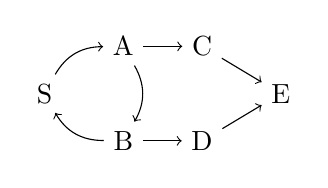
\begin{tikzpicture}
		\node (s) at (-1,0) {S};
		\node (a) at (0,0.6) {A};
		\node (b) at (0,-0.6) {B};
		\node (c) at (1,0.6) {C};
		\node (d) at (1,-0.6) {D};
		\node (e) at (2,0) {E};
		\draw[->, bend left] (s) to (a);
		\draw[->, bend left] (a) to (b);
		\draw[->, bend left] (b) to (s);
		\draw[->] (a) to (c);
		\draw[->] (b) to (d);
		\draw[->] (c) to (e);
		\draw[->] (d) to (e);
	\end{tikzpicture}
	\end{center}
	In Schritt~\ref{alg:unit-step-dg} wählen wir den Zykel $S \-> A \-> B \-> S$ und erhalten für $P'$ die folgenden den Regeln.
	\begin{align*}
		S &\-> C\mid D\ \mid 0S1S \mid 1S0S\\
		C &\-> E\\
		D &\-> E\\
		E &\-> \varepsilon\\
	\end{align*}
	Nach dem zweiten Anwenden von Schritt~\ref{alg:unit-step-dg} erhalten wir den folgenden gerichteten Graphen und wählen in Schritt~\ref{alg:unit-step-dag} die durch die Zahlen angedeutete topologische Sortierung.
	\begin{center}
	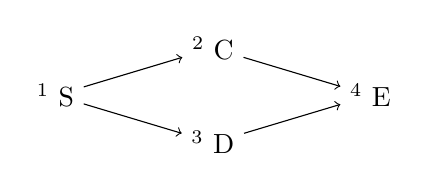
\begin{tikzpicture}
		\node (s) at (0,0) {$^1$ S};
		\node (c) at (2,0.6) {$^2$ C};
		\node (d) at (2,-0.6) {$^3$ D};
		\node (e) at (4,0) {$^4$ E};
		\draw[->] (s) to (c);
		\draw[->] (s) to (d);
		\draw[->] (c) to (e);
		\draw[->] (d) to (e);
	\end{tikzpicture}
	\end{center}
	Am Ende von Schritt~\ref{alg:unit-step-chain} sieht die Regelmenge $P'$ wie folgt aus.
	\begin{align*}
		S &\-> \varepsilon \mid 0S1S \mid 1S0S\\
		C &\-> \varepsilon\\
		D &\-> \varepsilon\\
		E &\-> \varepsilon\\
	\end{align*}

\end{Bsp}



\begin{Def}[name={[\acs*{CFG} in \acs*{CNF}]}]
	Eine \ac{CFG} $\mathcal{G} = (\Sigma, N, P, S)$ ist in \ac{CNF}, falls jede
  Regel die Form $A\->a$, $A\->BC$, oder $S \-> \Eps$ hat, wobei $A,B,C\in N$, $a\in\Sigma$.
  Falls $S \to \Eps \in P$, dann darf $S$ auf keiner rechten Seite einer Regel vorkommen.
\end{Def}
\begin{Satz}\label{satz:CFGtoCNF}
Es gibt einen Algorithmus der für eine \ac{CFG} $\mathcal{G}$ in $O(|\mathcal{G}|^3)$ Rechenschritten eine äquivalente \ac{CFG} $\mathcal{G}'$ in CNF mit $|\mathcal{G}'|\in O(|\mathcal{G}|^2)$ berechnet.
\end{Satz}

\begin{proof} (Beweisskizze)
	Ein Algorithmus der diese Eigenschaften erfüllt ist das Hintereinanderschalten von \textsc{Sep}, \textsc{Bin}, \textsc{Del} und \textsc{Unit}.\footnote{Es genügt sogar nur \textsc{Del} und dann \textsc{Unit} anzuwenden, da \textsc{Del} schon \textsc{Sep} und \textsc{Bin} ausführt.}
		\begin{itemize}
	\item Zur Korrektheit:
	
	Wir zeigen dass jedes dieser vier Verfahren die vom vorherigen Verfahren etablierte Eigenschaft nicht zerstört und dass die vier etablierten Eigenschaften für die \ac{CNF} hinreichend sind.
	
	\item Zu Laufzeit und Größe des Resultates:
	
	Die ersten drei Verfahren erhöhen die Größe der Grammatik nur linear und die Laufzeiten sind durch $O(|\mathcal{G}|^3)$ beschränkt. 
	Für \textsc{Unit} sind die in diesem Satz genannten Kosten eine obere Schranke. 
	\qedhere
	\end{itemize}
\end{proof}
	

\begin{lemma}
 Die Menge der Typ-2-Sprachen ist eine Teilmenge der Typ-1-Sprachen.
\end{lemma}
\begin{proof}
 Zu jeder Typ-2-Grammatik existiert eine äquivalente $\Eps$-freie Typ-2-Grammatik.
 Diese ist nach Definition auch eine Typ-1-Grammatik.
\end{proof}



% \begin{Beobachtung}
%   Ist $\mathcal{G} = (\Sigma, N, P, S)$ in \ac{CNF}, dann lassen sich für die Ableitungsbäume $\T \in \operatorname{Abl}(S)$ folgende Eigenschaften feststellen:
%   \begin{enumerate}
%   \item $\T$ ist ein Binärbaum. 
%   \item Falls $Y(\T) = w$, so ist die Anzahl der Blätter des Baumes $|w|$.
%   \qedhere
%   \end{enumerate}
% \end{Beobachtung}



\newcommand{\expl}[1]{{\color{blue} #1}}

\subsection{Wortproblem und Leerheitsproblem für kontextfreie Sprachen}
\begin{Satz}[name={[Wortproblem für \acs*{CFL} entscheidbar]}]
	Es gibt einen Algorithmus, für gegebene \ac{CFG} $\mathcal{G}$ in \ac{CNF} und gegebenes Wort $w$
	in $O(|w|^3\cdot |\mathcal{G}|)$ Schritten und mit $O(|w|^2\cdot |\mathcal{G}|)$ Speicherplatz
	entscheidet ob $w\in L(\mathcal{G})$ gilt.
\end{Satz}



\begin{proof}[\acsu{CYK}-Algorithmus] Sei $w = a_1\dots a_n\in\Sigma^*$.
	% Der \ac{CYK}-Algorithmus berechnet bei Eingabe von $\mathcal{G}$ und $w$, ob $w\in L(\mathcal{G})$.
	Der \ac{CYK}-Algorithmus aus \autoref{fig:AlgCYK} erfüllt diese Eigenschaften.
	Wir wollten zunächst die Idee des Algorithmus erklären.
	
	Definiere für $1\leq i < j\leq n$:
	\[
	M_{ij} = \{ A \in N \mid A \stackrel{*}{\vdash}_\mathcal{G} a_i\dots a_j \}\label{eqn:CykMatrixEintragDeriv}\tag{EntryDeriv}
	\]
	\expl{Wir definieren also Mengen von Nichtterminalsymbolen die sich schön als obere Dreiecksmatrix darstellen lassen.
		Die Matrix enthält einen Eintrag pro Teilwort von $w$, genauer der Eintrag $M_{ij}$ enthält das Nichtterminalsymbol $A$ 
		genau dann wenn wir von $A$ das Teilwort vom $i$-ten Zeichen bis zum $j$-ten Zeichen ableiten können.
		Zum Lösen des eigentlichen Problemes hilft dieses Vorgehen zunächst nichts.
		Urspünglich wollte wir wissen ob wir das Wort $W$ aus de Startsymbol ableiten können.
		Nun müssen wir diese Frage für alle Teilwörter und alle Nichtterminalsymbole beantworten.
	}
	
	Offensichtlich gilt: $w\in L(\mathcal{G})$ genau dann, wenn $S \stackrel{*}{\vdash}_\mathcal{G} w$ genau dann, wenn $S \in M_{1n}$.
	\expl{
		Zum Lösen des eigentlichen Problemes hilft uns das betrachten der Matrix also zunächst nicht.
		Urspünglich wollte wir wissen ob wir das Wort $W$ aus de Startsymbol ableiten können.
		Nun müssen wir diese Frage für alle Teilwörter und alle Nichtterminalsymbole beantworten.
	}
	\begin{align*}
		\intertext{Es gilt für $i=j$}
		M_{ii} &= \{A \mid A\-> a_i \in P\} \\
		\intertext{
			\expl{Die Einträge auf der Hauptdiagonalen hängen also nur von Regeln der Form $A \to a$ 
				ab und wir können diese Einträge jeweils durch einmaliges Iterieren über alle Regeln bestimmen.}
		}
		\intertext{Es gilt für $i<j$}
		M_{ij} &= \{ A \mid A\-> BC \in P \text{ und } BC \stackrel{*}{\vdash}_{\mathcal{G}} a_i\dots a_j \}\\
		&= \{ A \mid A\-> BC\in P \text{ und } \exists k \in\{i, \ldots j-1\} \text{ sodass }
		\begin{aligned}[t]
			B &\stackrel{*}{\vdash}_{\mathcal{G}} a_i\dots a_k \text{ und } C \stackrel{*}{\vdash}_{\mathcal{G}} a_{k+1}\dots a_j \}
		\end{aligned}\\
		&= \{ A \mid A\-> BC\in P \text{ und } \exists k \in\{i, \ldots j-1\} \text{ sodass } B\in M_{ik} \text{ und } C \in M_{(k+1)j}\}
		% &= \bigcup_{k=i}^{j-1} \{ A \mid A \-> BC \land 
		% 	\begin{aligned}[t]
		% 		B &\xRightarrow{*} a_i\dots a_k \land{}\\
		% 		C &\xRightarrow{*} a_{k+1}\dots a_j \}
		% 	\end{aligned}\\
		% &= \bigcup_{k=i}^{j-1} \{ A \mid A \-> BC \land B \in M_{i,k} \land C \in M_{k+1,j} \}
	\end{align*}
	
	\expl{
		Wir können also die Berechnung der Matrixeinträge die nicht auf der Hauptdiagonalen liegen 
		auf die Existenz bestimmter Regel der Form $A\-> BC$ und Inhalte bestimmter anderer Matrixeinträge zurückführen.
	}
	
	Beobachtung: Der Wert von $M_{ij}$ hängt nur von $M_{i'j'}$ mit $i'>i, j'\leq j$ oder $i'\geq i,j'<j$ ab.
	Wir können die $M_{ij}$ also mit dem Verfahren aus \autoref{fig:AlgCYK} berechnen.
	
	\expl{
		Es gibt also insbesonere keine zyklischen Abhängigkeiten und bei geeigneter Iterationsreihenfolge 
		über alle Matrixeinträge kann jeder Eintrag direkt mit Hilfe der Einträge aus vorherigen
		Iterationen bestimmt werden.
	}
	% \medskip
	
	Skizze der verbleibenden Beweisschritte.
	
	Zur Korrektheit: Zeige via einer verschachtelten Induktion über Zeilen und Spalten, 
	dass am Ende der zweiten for-Schleife für alle $M_{i'j'}$ mit $i'\in\{i,\ldots, n-1\}$ und $j'\in\{i+1,\ldots, j\}$
	die oben definierte Gleichung (\ref{eqn:CykMatrixEintragDeriv}) gilt.
	
	Zur Laufzeitabschätzung: Die Iterationen jeder for-Schleife sind durch die Länge des Wortes $|w|$ beschänkt. 
	In der innersten Schleife genügt es ein mal über die Regeln der Grammatik zu iterieren.
	
	Zum Speicherplatz: Wir benötigen weniger als $|w|^2$ Matrixeinträge 
	und jeder Eintrag enthält höchtens alle Variablen die in Regeln der Grammatik vorkommen.
	\qedhere
\end{proof}


\begin{figure}
	\small
	% \framebox[\textwidth]{
	% \parbox{0.95\textwidth}{
	\begin{description}
		\item[Eingaben:] \ac{CFG} $\mathcal{G} = (\Sigma, N, P, S)$ in CNF und Wort $a_1\ldots a_n\in\Sigma^*$
		\item[Ausgabe:] ``Ja'' falls $a_1\ldots a_n\in L(\mathcal{G})$, ``Nein'' sonst.
	\end{description}
	
	Sei $M$  eine $n\x n\text{-Matrix mit (initial) } M_{ij}=\varnothing \text{ für alle } i, j$  // $O(n^2)$
	
	\begin{center}
		\begin{minipage}{12cm}
			\begin{lstlisting}[mathescape,morekeywords={for,do,return},morecomment={[l]{//}}]
for i=1 .. n do  // $O(|\mathcal{G}|)\cdot O(n)$
  $M_{ii}=\{A \mid A \-> a_i \}$
for i=n-1 .. 1 do
  for j=i+1 .. n do
    for k=i .. j-1 do  // $O(|\mathcal{G}|)\cdot O(n^3)$
      $M_{ij}=M_{ij}\cup \{ A \mid A \-> BC, B\in M_{ik}, C\in M_{(k+1)j} \}$
return $S\in M_{1n}$
			\end{lstlisting}
			\qedherefixlstlisting
		\end{minipage}
	\end{center}
	%   }
	% }
	
	\caption{CYK Algorithmus}
	\label{fig:AlgCYK}
\end{figure}


\begin{Bsp}
	Sei $\Sigma=\{a,b,c\}$.\
	Betrachte das Wort $w=aaabbbcc$ und die \ac{CFG} $\mathcal{G} = (\Sigma, \{S,X,Y\}, P, S)$\footnote{
		Es gilt $L(\mathcal{G})=\{a^nb^nc^m \mid n,m\geq 1\}$ 
		aber das bestimmen der erzeugten Sprache ist für das Entscheiden des Wortproblemes 
		natürlich nicht erforderlich.}
	deren Regeln $P$ wie folgt definiert sind.
	\begin{align*}
		S &\-> XY\\
		X &\-> ab \mid aXb\\
		Y &\-> c \mid cY
	\end{align*}
	Damit wir den \ac{CYK} Algorithmus anwenden können transformieren wir $\mathcal{G}$ in eine äquivalente Grammatik in CNF.
	Z.B. in die \ac{CFG} $\mathcal{G'} = (\Sigma, \{S, X, Y, Z, A, B, C\}, P', S)$, deren Regeln $P'$ wie folgt definiert ist.
	\begin{align*}
		S &\-> XY\\
		X &\-> AB \mid AZ\\
		Z &\-> XB\\
		Y &\-> CY | c\\
		A &\-> a, B \-> b, C \-> c
	\end{align*}
	Wir wenden den CYK Algorithmus an und erhalten die folgende Matrix.
	

	
	\begin{minipage}{0.6\textwidth}
	\begin{center}
		\begin{tabular}[t]{M{c}|*8{M{c}|}}
			%       w = & a & a & a & b & b & b & c & c \\
			\cline{2-9}
			% 			M =
			& A               & \bullet & \bullet & \bullet & \bullet & X ~\text{\tiny 6}& \emph{S} ~\text{\tiny 7}& S~\text{\tiny 8}       \\
			\cline{2-9}
			\multicolumn{1}{r@{}}{a} & & A       & \bullet & \bullet & {X} ~\text{\tiny 4}& {Z} ~\text{\tiny 5}& \bullet & \bullet \\
			\cline{3-9}
			\multicolumn{1}{c}{} & \multicolumn{1}{r@{}}{a} &    & A       & X ~\text{\tiny 2}      & Z     ~\text{\tiny 3}  & \bullet & \bullet & \bullet \\
			\cline{4-9}
			\multicolumn{2}{c}{} & \multicolumn{1}{r@{}}{a} &         & B       & \bullet & \bullet & \bullet & \bullet \\
			\cline{5-9}
			\multicolumn{3}{c}{} & \multicolumn{1}{r@{}}{b} &              & B       & \bullet & \bullet & \bullet \\
			\cline{6-9}
			\multicolumn{4}{c}{} & \multicolumn{1}{r@{}}{b} &                   & B & \bullet & \bullet \\
			\cline{7-9}
			\multicolumn{5}{c}{} & \multicolumn{1}{r@{}}{b} &                        & C,Y     & Y ~\text{\tiny 1}      \\
			\cline{8-9}
			\multicolumn{6}{c}{} & \multicolumn{1}{r@{}}{c} &                              & C,Y     \\
			\cline{9-9}
			\multicolumn{7}{c}{} & \multicolumn{1}{r@{}}{c} & \multicolumn{1}{c}{}
		\end{tabular}
	\end{center}
	\end{minipage}
	\begin{minipage}{0.5\textwidth}
	\end{minipage}
	\begin{minipage}{0.35\textwidth}
		Zellen, die mit "`${\bullet}$"' markiert sind, sind leer.
		Die Reihenfolge, in der die nicht-diagonalen, nicht leeren Zellen eingetragen wurden, ist mit kleinen Zahlen markiert.
		Beispielsweise wurde $M_{35} = \{Z\}$ mit Zahl "`{\scriptsize 3}"' \emph{nach} $M_{78} = \{Y\}$ mit Zahl "`{\scriptsize 1}"' eingetragen.
	\end{minipage}

	Da $S \in M_{1n}$, gilt $w \in L(\mathcal{G}')$.
\end{Bsp}


\begin{Korollar}
	Es gibt einen Algorithmus, für gegebene \ac{CFG} $\mathcal{G}$ und gegebenes Wort $w$
	in $O(|w|^3\cdot |\mathcal{G}|^2)$ Schritten und mit $O(|w|^2\cdot |\mathcal{G}|^2)$ Speicherplatz
	entscheidet ob $w\in L(\mathcal{G})$ gilt.
\end{Korollar}

\begin{proof}
	Aus \autoref{satz:CFGtoCNF} wissen wir dass eine \ac{CFG} in \ac{CNF} 
	konvertieren können sodass deren Größe höchstens quadratisch wächst.
	Anschließend wenden wir den CYK Algorithmus auf das Resultat an.
\end{proof}

\expl{
Um \datenote{12.12.2018} möglichst schnell zum Unterkapitel über Typ-3-Sprachen zu kommen wurde das restliche Unterkapitel in der Freitagsvorlesung übersprungen.
}

\begin{Satz}[name={[Entscheidbarkeit des Leerheitsproblems für kontextfreie Sprachen]}]
  \label{thm:cfl-decidable-emptyness}
    Es gibt einen Algorithmus, der das Leerheitsproblem%
    \footnote{Gefragt ist, ob $L(\mathcal{G}) = \{ w\in\Sigma^* \mid S\overset{*}{\vdash} w \} \overset{?}{=} \varnothing$.}
    für kontextfreie Sprachen in $O(|\mathcal{G}|)$ entscheidet.
\end{Satz}

\begin{Def}
	Sei $\mathcal{G} = (\Sigma, N, P, S)$ eine beliebige Grammatik. 
	Wir nennen ein Nichtterminalsymbol $A\in N$ co-erreichbar falls es ein Wort $w\in\Sigma$ existiert, 
	sodass $A \stackrel{*}{\vdash}_\mathcal{G} w$ gilt.
	\expl{Ein Symbol ist also co-erreichbar genau dann wenn wir daraus irgendein Wort ableiten können.}
\end{Def}


\begin{proof}
    Sei $\mathcal{G} = (\Sigma, N, P, S)$ eine \ac{CFG} für $L$.
    Wir definieren die Menge $M$ der co-erreichbaren Nichtterminalsymbole.
    %
    $$M = \{ A \mid A \stackrel{*}{\vdash}_\mathcal{G} w, w\in \Sigma^* \}$$
    %
    Offensichtlich gilt: $L =\varnothing \<=> S\notin M$.
    
    Wir können $M$ induktiv berechnen. Wir definieren hierfür:
	\begin{align*}
		M_0 &= \{ A \mid A \-> w\in P, w\in \Sigma^* \}\\
		M_{i+1} &= M_i\cup \{ A \mid A \-> \alpha\in P, \alpha\in(\Sigma\cup M_i)^* \}
	\end{align*}
    Offensichtlich gilt für alle $i\in\N$ $M_i\subseteq M_{i+}$ und $M_i\subseteq M$.
    Da $M\subseteq N$ endlich ist, gibt es ein $n$, sodass $M_n = M_{n+1}$ (hier ohne Beweis).
    
    Wir können daher $M$ analog zu $\operatorname{Nullable}(\mathcal{G})$ (siehe \autoref{satz:3.nullable}) in $O(|\mathcal{G}|)$ berechnen.
\end{proof}
\begin{Bem}
        Wenn wir in einer Grammatik $\mathcal{G}$ ein nicht co-erreichbares Nichtterminalsymbol (und alle zugehörigen Regeln) entfernen, ändert sich $L(\mathcal{G})$ nicht.
        Wir können eine gegebene Grammatik also optimieren, indem wir alle nicht co-erreichbaren Nichtterminalsymbole entfernen.
\end{Bem}
% \begin{Satz}[name={[Entscheidbarkeit des Endlichkeitsproblem für \acs*{CFL}]}]
% 	Das Endlichkeitsproblem für kontextfreie Sprachen ist entscheidbar.
% \end{Satz}
% \begin{proof}
% 	Mit \ac{PL} analog zum Endlichkeitsproblem für reguläre Sprachen (Prüfe, ob $\exists w \in L$ mit $n < |w| \le 2n$).
% 	Die Grundidee ist: $L$ ist endlich genau dann, wenn es keinen (echt wachsenden) Zyklus gibt, der zu einer Wortbildung beitragen kann.
% \end{proof}


\subsection{Einschub: Typ-3-Sprachen}
\begin{Satz}[name={[Typ-3-Sprache ist regulär]}]
	$L$ ist regulär \<=> $L$ ist Typ-3-Sprache.
\end{Satz}
\begin{proof}
	\begin{description}[font=\normalfont,labelwidth=\widthof{"'\=>"':},leftmargin=!]
	\item["`\=>"'] Sei $\A =(\Sigma, Q,\delta,\qinit,F)$ \ac{DEA} für $L$.\\
		Konstruiere Typ-3-Grammatik $\mathcal{G}=(\Sigma,N,P,S)$ mit
		\begin{align*}
		 N &= Q\\
		 S &= \qinit\\
		 P &= \{ q\rightarrow aq'\mid q,q'\in Q, a\in\Sigma, \delta(q,a)=q'\}\cup \{ q\rightarrow\Eps\mid q\in F\}
		\end{align*}
		Es gilt $L(\mathcal{G})=L(\A)$. (ohne Beweis)
	\item["`\<="'] Sei $\mathcal{G}=(\Sigma,N,P,S)$ Typ-3-Grammatik.
	Dann erhalten wir durch Anwenden von \textsc{Bin} eine äquivalente Grammatik, in der jede Regel eine der folgenden Formen hat:
	  \begin{alignat*}{3}
	 A &\-> \Eps && \quad \text{für } A\in N\\[0.5mm]
   A &\-> a && \quad \text{für } A\in N, a\in\Sigma\\[0.5mm]
   A &\-> a_1a_2 && \quad \text{für } A\in N, a_1,a_2\in\Sigma\\[0.5mm]
   A &\-> aB && \quad \text{für } A\in N, a\in\Sigma, B\in N
  \end{alignat*}
  Wir machen nun die folgenden Modifikationen.
  \begin{itemize}
   \item Wir fügen eine frische Variable $Y_{\Eps}$ und die Regel $Y_{\Eps}\rightarrow\Eps$ hinzu.
   \item Wir löschen jede Regel der zweiten Form und führen stattdessen die Regel $A \-> aY_{\Eps}$ ein.
  \item Wir löschen jede Regel der dritten Form und führen stattdessen eine frische Variable $Y_{a_2}$ und die Regeln $A \-> a_1Y_{a_2}$ und $Y_{a_2} \-> a_2Y_\Eps$ ein.
  \end{itemize}
	Die resultierende Grammatik $\mathcal{G}=(\Sigma,N',P',S)$ ist äquivalent zu $\mathcal{G}$. (Ohne Beweis)

	Wir konstruieren nun den folgenden NEA. $\calN=(\Sigma,Q,\delta,\qinit,F)$
	\begin{alignat*}{2}
		Q &=N'\\
		B\in\delta(A,a) & \text{ \  gdw \ } A\rightarrow aB \in P'\\
		\qinit &=S\\
		F &= \{ A\in N'\mid A\rightarrow\Eps\in P'\}
	\end{alignat*}
		Es gilt $L(\mathcal{G})=L(\A)$. (ohne Beweis) \qedhere

	\end{description}
\end{proof}


\begin{lemma}
	$\mathcal{M}_3 \subsetneq \mathcal{M}_2$ (d.h., die regulären Sprachen sind eine \emph{echte} Teilmenge der kontextfreien Sprachen).
\end{lemma}
\begin{proof}
	Betrachte $L_\text{centered}=\{0^n10^n \mid n\in\N \}\subseteq\{0,1\}^*$\\
	Sowohl aus \autoref{bsp:2.centeredMyhillNerode} als auch aus \autoref{bsp:2.centeredPL} ist bekannt, 
	dass $L_\text{centered}$ nicht regulär ist.
	Es gibt aber eine Typ-2-Grammatik für $L_\text{centered}$:
	\[ \mathcal{G} = (\{0,1\}, \{S\}, \{S\->1, S\->0S0 \}, S) \]
	(ohne Beweis)
\end{proof}





\hide{


\subsection{Abschlusseigenschaften für kontextfreie Sprachen}


\begin{Satz} % 4.7
  \label{thm:cfl-closed-reg-intersect}
	Die Menge \acs{CFL} ist abgeschlossen unter $\cup, \cdot, ^*$, jedoch \emph{nicht} unter $\cap, \overline{\phantom{A}}$.
\end{Satz}
\begin{proof}
	\begin{align*}
		\mathcal{G}_i :&= (N_i, \Sigma,P_i,S_i) \quad i=1,2\\
		\text{"`}\cup\text{"'}: N &= N_1\dotcup N_2\dotcup\{S\}\\
		P &= \{S\->S_1, S\->S_2 \} \cup P_1\cup P_2\\
		\text{"`}\cdot\text{"'}:: N &= N_1\dotcup N_2\dotcup\{S\}\\
		P &= \{ S\->S_1S_2 \} \cup P_1\cup P_2\\
		\text{"`}^*\text{"'}: N &= N_1 \dotcup \{S\}\\
		P &= \{ S\->\Eps, S\-> S_1S \} \dotcup P_1
	\end{align*}
	\begin{itemize}
	\item für $n\geq 1$
		\[ \underbrace{\{a^nb^nc^n\}}_{\notin \acs{CFL}} = \underbrace{\{a^nb^nc^m \mid n,m\geq 1 \}}_{\in \acs{CFL}} \cap \underbrace{\{a^mb^nc^n \mid m,n\geq 1 \}}_{\in \acs{CFL}} \]
		Also \ac{CFL} nicht abgeschlossen unter $\cap$.
	\item Angenommen CFL wäre abgeschlossen unter $\overline{\phantom{X}}$\\
		Falls $L_1,L_2\in \acs*{CFL}$, dann ist $\overline{L}_1,\overline{L}_2\in\acs*{CFL}$ nach Annahme.\\
		$\curvearrowright \overline{L}_1\cup \overline{L}_2\in\acs*{CFL}$ wegen Teil "'$\cup$"'.\\
		$\curvearrowright \overline{\overline{L}_1\cup \overline{L}_2} = L_1\cap L_2\in\acs*{CFL}\ \lightning$ zu Teil "'$\cap$"'. \qedhere
	\end{itemize}
\end{proof}








\datenote{14.12.16}
\begin{Satz} % 4.8
	Die Menge \ac{CFL} ist abgeschlossen unter "`$\cap$ mit regulären Sprachen REG"'.
  Das heißt, für alle $L \in \mathrm{CFL}$ und $R \in \mathrm{REG}$ gilt $L \cap R \in \mathrm{CFL}$.
\end{Satz}
\begin{proof}
  Sei $\mathcal{G} = (\Sigma, N, P, S)$ kontextfreie Grammatik in \ac{CNF} mit $L(\mathcal{G}) = L$.

  Sei $M = (Q, \Sigma, q, \delta, q_0, F)$ NEA mit $L(M) = R$.

  Definiere $\mathcal{G}' = (N', \Sigma, P', S)$ durch
  \begin{itemize}
  \item[] $N' = Q \times N \times Q \cup \{S\}$
  \item[] $P' =
    \begin{aligned}[t]
      &\{ (p, A, q) \to a \mid A \to a \in P \text{ und } \delta(p,a) \ni q \} \\
      &\cup \{ (p, A, q) \to (p,B,q')(q',C,q) \mid A \to BC \in P \text{ und } p,q,q' \in Q\} \\
      &\cup \{ S \to (q_0, S, q) \mid q \in F \}
    \end{aligned}
    $
  \end{itemize}
  Durch die $S \to \ldots$ Regeln erzeugt $\mathcal{G}'$ offensichtlich genau die Wörter, die durch die Nichtterminalsymbole $(q_0, S, q)$ für $q \in F$ erzeugt werden.
  Es bleibt zu zeigen, dass ein Nichtterminal genau die Wörter aus $L$ erzeugt die gleichzeitig einen (akzeptierenden) Lauf $q_0\ldots q$ von $M$ erlauben.
  Wir zeigen eine Verallgemeinerung: für alle $p,q \in Q$ und $A \in N$ gilt
  \begin{align*}
    &(p,A,q) \stackrel{*}{\Longrightarrow}_{\mathcal{G}'} w \\
    \text{ gdw } & A \stackrel{*}{\Longrightarrow}_{\mathcal{G}} w \text{ und es existiert ein Lauf } p\ldots q \text{ von $M$ auf $w$}
  \end{align*}
  \begin{itemize}
  \item Richtung "`links nach rechts"': (siehe Übung)
  \item Richtung "`rechts nach links"':

    Per Induktion über den Ableitungsbaum $\mathcal{A} = \pi(\mathcal{A}_1,\ldots,\mathcal{A}_n) \in \operatorname{Abl}(\mathcal{G}, A)$ mit $Y(\mathcal{A}) = w$.
    \begin{description}
      \item[IV] $\forall 1 \le i \le n:$ wenn $w_i = Y(\mathcal{A}_i)$ mit $\mathcal{A}_i \in \operatorname{Abl}(\mathcal{G}, A_i)$ und es existiert ein Lauf  $p_i\ldots q_i$  von M auf $w_i$, dann $(p_i, A_i, q_i) \stackrel{*}{\Longrightarrow}_{\mathcal{G}'} w_i$.
      \item[IS] \hfill
        \begin{itemize}
        \item $\pi = A \to a$, $a \in \Sigma$.
          Es gilt $w = a$ und $pq$ ist Lauf auf $a$.
          Folglich ist $\delta(p, a) \ni q$. Damit ist $(p,A,q) \to a \in P'$, woraus direkt folgt, dass $(p,A,q) \Longrightarrow_{\mathcal{G}'} a$.
        \item $\pi = A \to BC$, $\mathcal{A} = \pi(\mathcal{A}_1, \mathcal{A}_2)$, $Y(\mathcal{A}_1) = w_1$, $Y(\mathcal{A}_2) = w_2$, \mbox{$\mathcal{A}_1 \in \operatorname{Abl}(\mathcal{G}, B)$} und $\mathcal{A}_2 \in \operatorname{Abl}(\mathcal{G}, C)$.

          Es gilt $w = w_1w_2$ und $\zeta = p\ldots q$ ist Lauf auf $w_1w_2$.
          Es existiert also $q'$ sodass $\zeta = p\ldots q' \ldots q$ und $p\ldots q'$ ist Lauf auf $w_1$ und $q' \ldots q$ ist Lauf auf $w_2$.

          Es folgt nach IV, dass
          \begin{displaymath}
            (p, B, q') \stackrel{*}{\Longrightarrow}_{\mathcal{G}'} Y(\mathcal{A}_1) = w_1 \text{ und } (q', C, q) \stackrel{*}{\Longrightarrow}_{\mathcal{G}'} Y(\mathcal{A}_2) = w_2.
          \end{displaymath}
          Nun ist $(p,A,q) \to (p,B,q')(q',C,q) \in P'$ nach Konstruktion, also ist folgende Ableitung möglich:
          \begin{displaymath}
            (p,A,q) \Longrightarrow_{\mathcal{G}'} (p,B,q')(q',C,q) \stackrel{*}{\Longrightarrow}_{\mathcal{G}'} w_1(q',C,q) \stackrel{*}{\Longrightarrow}_{\mathcal{G}'} w_1w_2 = w
          \end{displaymath}
        \end{itemize}
    \end{description}
  \end{itemize}
  \end{proof}
%
%Zuletzt: $\acsu{CFL}\land\acsu{REG}=\ac{REG}$
\begin{Satz}[name={[$L\subseteq R$ entscheidbar]}] %\rlwarning{Satz 4.9}
	Sei $L\in\ac{CFL}$ und $R\in\textrm{REG}$. Es ist entscheidbar, ob $L\subseteq R$.
\end{Satz}
\begin{proof}
  Es gilt $L\subseteq R \text{ gdw } L \cap\overline{R} = \emptyset$.

  Da $R \in \mathrm{REG}$ ist durch die Abschlusseigenschaften regulärer Sprachen auch $\overline{R} \in \mathrm{REG}$.
  Nach Satz \ref{thm:cfl-closed-reg-intersect} ist $L \cap\overline{R} \in \mathrm{CFL}$.
  Nach Satz \ref{thm:cfl-decidable-emptyness} ist $L \cap\overline{R} = \emptyset$ daher entscheidbar
\end{proof}


\draftnote{25.11.16}


\datenote{30.11.16}


\datenote{2.12.16}


\subsection{Das Pumping Lemma für kontextfreie Sprachen}
\begin{Satz}[Pumping lemma für \acs*{CFL}, uvwxy Lemma]
\label{satz:PL für CFL}
%\rlnote{Satz \# 4.2?}
	Sei $L\in {CFL}$. Dann $\exists n>0$, sodass $\forall z\in L$ mit $|z|\geq n\ \exists u,v,w,x,y$ sodass $z=uvwxy$ mit
	\begin{itemize}
	\item $|vwx|\leq n$
	\item $|vx|\geq 1$
	\item $\forall i \in \N : uv^iwx^iy\in L$
	\end{itemize}
\end{Satz}
\begin{proof}
	Sei $\mathcal{G}= (\Sigma,N,P,S)$ in \ac{CNF} mit
    $L(\mathcal{G}) = L$. Wähle die Pumping-Konstante $n=2^{|N|}$.
    
     Betrachte den Ableitungsbaum $\mathcal{A} \in \operatorname{Abl}(\mathcal{G}, S)$ von $z$ mit $|z|\geq n$. 
    \footnote{Intuition: Da $\mathcal{G}$ in \ac{CNF}, ist Ableitungsbaum $\mathcal{A}$ ein Binärbaum. 
        Mit $|N|$ 
    verschiedenen Nichtterminalsymbolen kann man 
    also maximal Wörter der Länge $2^{|N|}$ ableiten, wenn man keine Ableitung doppelt nutzen möchte. 
    Leitet man ein längeres Wort ab, so muss man mind. eine Ableitung doppelt nutzen.
     Dann kann man sie aber auch gleich $i$-fach nutzen ($v^i$ und $x^i$), und ist immernoch in der Sprache.}
  $\mathcal{A}$ ist ein Binärbaum mit $|z|\geq n = 2^{|N|}$ Blättern. In einem solchen Binärbaum existiert ein Pfad $\zeta$ der Länge $\geq |N|$.
	Auf $\zeta$ liegen $\geq |N|+1$ \acfp{NT}, es muss also mindestens ein Nichtterminal $A$ mehrmals vorkommen.
	
  Folge $\zeta$ vom Blatt Richtung Wurzel und bis sich das ein $A$ das erste Mal wiederholt. Das geschieht nach $\le |N|$ Schritten.
  Nun teile $z = uvwxy$ wie hier skizziert:
  
			\begin{tikzpicture}[>=stealth,
				widebox/.style={draw, minimum width=.75cm, minimum height=.35cm, inner sep=0pt}
				,dot/.style={inner sep=0pt,outer sep=0pt,label={center:\scalebox{.75}{\textbullet}}}
				]
				
				\node[dot,label={above right:$S$}] (v1) at (0,-1) {};
				\node[dot] (v2) at (-0.25,-1.6) {};
				\node[dot,] (v3) at (0,-2) {};
				\node[dot] (v4) at (-0.5,-2.5) {};
				\node[dot,label={above right:$A$}] (v5) at (0,-3) {};
				\node[widebox] (v6) at (-1.5,-3.5) {$u$};
				\node[widebox] (v7) at (-.75,-3.5) {$v$};
				\node[widebox] (v8) at (0,-3.5) {$w$};
				\node[widebox] (v9) at (.75,-3.5) {$x$};
				\node[widebox] (v10) at (1.5,-3.5) {$y$};
				
				\draw  (v1) edge (v2);
				\draw  (v2) edge (v3);
				\draw  (v3) edge (v4);
				\draw  (v4) edge (v7.north west);
				\draw  (v4) edge (v5);
				\draw  (v3) edge (v10.north west);
				\draw  (v5) edge (v8.north west);
				\draw  (v5) edge (v8.north east);
				\draw  (v1) edge (v6.north west);
				\draw  (v1) edge (v10.north east);
				\node[align=left, text height=3em,inner sep=2pt] at (2.1,-1.5) {$A\rightarrow BC$~\small{ist Binärbaum}} edge[->,shorten >=.1cm] (v3);
				\node[inner sep=0pt] at (2.75,-3.5) {$A\rightarrow a$} edge[->] (v10);
				\node (v11) at (0,-4) {$z$};
				\draw[semithick]
				let \p1 = (v6.west), \p2 = (v11), \p3 = (v10.east) in 
				 (\x1,\y2) edge[{Bar[]<}-] (v11) (v11) edge[-{>Bar[]}] (\x3,\y2);
			\end{tikzpicture}
	
      Nun gilt
      \begin{itemize}
      \item $|vx|\geq 1$, da $\zeta$ entweder durch $B$ oder durch $C$ läuft. Nehme also an, $\zeta$ verläuft durch $B$.
        Somit muss $C \stackrel{*}{\Longrightarrow} x$. In \ac{CNF} ist $C \stackrel{*}{\Longrightarrow} \Eps$ nicht möglich und somit ist $|x| \ge 1$.
        Der Fall, das $\zeta$ durch $C$ verläuft, ist analog.
      \item $|vwx| \le 2^{|N|} = n$ TODO
      \end{itemize}
		\begin{figure}[H]\centering
		\begin{subfigure}[b]{.29\linewidth}\centering
			\begin{tikzpicture}[node distance=.75cm, on grid,
					every node/.style={
						execute at begin node=$,
						execute at end node=$
					}
				]
				\node (0) {};
				\node (A1) [below=of 0] {A};
				\node (A2) [below=of A1] {A};
				\node (A3) [below=of A2] {A};
				
				\newlength\Offset \setlength\Offset{.75cm}
				\coordinate(p1) at ($(A2.south) - (0,\Offset)$);
				%
				\coordinate (A2l) at ($(p1) - (\Offset,0)$);
				\coordinate (A1l) at ($(A2l) - (\Offset,0)$);
				\coordinate (0l) at ($(A1l) - (\Offset,0)$);
				%
				\coordinate (A2r) at ($(p1) + (\Offset,0)$);
				\coordinate (A1r) at ($(A2r) + (\Offset,0)$);
				\coordinate (0r) at ($(A1r) + (\Offset,0)$) ;
				
				\coordinate (A3l) at ($(A3.south) - (\Offset,\Offset)$);
				\coordinate (A2l2) at ($(A3l) - (\Offset,0)$);
				%
				\coordinate (A3r) at ($(A3.south) + (\Offset,-\Offset)$);
				\coordinate (A2r2) at ($(A3r) + (\Offset,0)$);
				
				\node (dots) [below=\Offset of A3] {\vdots};
				
				\node (A4) [below=\Offset of dots] {A};
				\coordinate (A4l) at ($(A3l) - (0,2*\Offset)$);
				\coordinate (A4r) at ($(A3r) - (0,2*\Offset)$);
				
				\draw (0.south) edge (0l.center) edge (0r.center)
					(A1.south) edge (A1l.center) edge (A1r.center)
					(A2.south) edge (A2l2.center) edge (A2r2.center)
					(A3.south) edge (A3l.center) edge (A3r.center)
					(A4.south) edge (A4l.center) edge (A4r.center)
				;
				\draw (0l.center) edge node[below] {u} (A1l.center)
					(A1l.center)  edge node[below] {v} (A2l.center)
					(A2r.center)  edge node[below] {x} (A1r.center)
					(A1r.center)  edge node[below] {y} (0r.center)
					(A2l2.center) edge node[below] {v} (A3l.center)
					(A3r.center)  edge node[below] {x} (A2r2.center)
					(A4l.center)  edge node[below] {w} (A4r.center)
				;
			\end{tikzpicture}
			\caption{$uv^iwx^iy\in L$}
		\end{subfigure}
		\begin{subfigure}[b]{.28\linewidth}\centering
			\begin{tikzpicture}[node distance=.5cm, on grid,
					every node/.style={
						execute at begin node=$,
						execute at end node=$
					},
					widebox/.style={draw, minimum width=.75cm, minimum height=.35cm, inner sep=0pt}
				]
				\node (S) {S};
				\node[inner sep=2pt] (A) [below=of S.south, xshift=.2cm] {A};
				\coordinate (Ap) at (A.south west);
				\node[widebox] (w) [below=of Ap] {w};
				\node[widebox] (u) at ($(Ap)!2!(w.north west)+.5*(-.75,-.3)$) {u};
				\node[widebox] (y) at ($(Ap)!2!(w.north east)+.5*(.75,-.3)$) {y};
				
				\draw (S.south) edge (u.north west) edge (y.north east)
					(Ap) edge (u.north east) edge (y.north west) edge (w.north)
					($(S.south) - (.25,.6)$) edge (S.south) edge (Ap)
				;
			\end{tikzpicture}
			\caption{$\curvearrowright uwy\in L$}
		\end{subfigure}
		\begin{subfigure}[b]{.33\linewidth}\centering
			\begin{tikzpicture}[>=stealth,
				widebox/.style={draw, minimum width=.75cm, minimum height=.35cm, inner sep=0pt}
				,dot/.style={inner sep=0pt,outer sep=0pt,label={center:\scalebox{.75}{\textbullet}}}
				]
				
				\node[dot,label={above right:$S$}] (v1) at (0,-1) {};
				\node[dot] (v2) at (-0.25,-1.6) {};
				\node[dot,label={above right:$A$}] (v3) at (0,-2) {};
				\node[dot] (v4) at (-0.5,-2.5) {};
				\node[dot,label={above right:$A$}] (v5) at (0,-3) {};
				\node[widebox] (v6) at (-1.5,-3.5) {$u$};
				\node[widebox] (v7) at (-.75,-3.5) {$v$};
				\node[widebox] (v8) at (0,-3.5) {$w$};
				\node[widebox] (v9) at (.75,-3.5) {$x$};
				\node[widebox] (v10) at (1.5,-3.5) {$y$};
				
				\draw  (v1) edge (v2);
				\draw  (v2) edge (v3);
				\draw  (v3) edge (v4);
				\draw  (v4) edge (v7.north west);
				\draw  (v4) edge (v5);
				\draw  (v3) edge (v10.north west);
				\draw  (v5) edge (v8.north west);
				\draw  (v5) edge (v8.north east);
				\draw  (v1) edge (v6.north west);
				\draw  (v1) edge (v10.north east);
				\node[align=left, text height=3em,inner sep=2pt] at (2.1,-1.5) {$A\rightarrow BC$\small{ist Binärbaum}} edge[->,shorten >=.1cm] (v3);
				\node[inner sep=0pt] at (2.75,-3.5) {$A\rightarrow a$} edge[->] (v10);
				\node (v11) at (0,-4) {$z$};
				\draw[semithick]
				let \p1 = (v6.west), \p2 = (v11), \p3 = (v10.east) in 
				 (\x1,\y2) edge[{Bar[]<}-] (v11) (v11) edge[-{>Bar[]}] (\x3,\y2);
			\end{tikzpicture}
			\caption{$\exists$ Pfad mit Länge $\geq k$}
		\end{subfigure}
		\caption{Schema zu \autoref{satz:PL für CFL}}
	\end{figure}\vspace{-2em}\qedhere
\end{proof}

\begin{lemma} %\rlnote{Lemma \# 4.3?}
	$\mathcal{L}_2 \subsetneq \mathcal{L}_1$
\end{lemma}
\begin{proof}
	Sei $L=\{L=\{a^nb^nc^n \mid n\geq 1\}$.\\
	$L$ ist nicht kontextfrei. Verwende \ac{PL}. Angenommen $L$ sei kontextfrei.
	Sei dann $n$ die Konstante aus dem \ac{PL}.
	
	Wähle $z=a^nb^nc^n$ und somit $|z| = 3n \ge n$.
  Nach PL ist $z = uvwxy$ mit $|vx| \ge 1$ und $|vwx| \le n$.

  Durch $|vwx| \le n$ ergeben sich folgende Möglichkeiten:
  \begin{itemize}
  \item $vwx = a^j$: 
    Für $i=0$ ist $vwx=w$ mit $|w| < j$.
    Anzahl der $a$ stimmt nicht mehr mit $n$ überein.
  \item $vwx = a^kb^j$:
    \begin{itemize}
    \item Falls $v = a^{k'}$, $x = b^{j'}$: Für $i=0$ stimmt die Anzahl der $a$ nicht mehr mit $n$ überein.
    \item Falls $v$ ein Gemisch aus $a$ und $b$ enthält.
      Für $i\ge 2$ würde eine Folge $a^n$ durch eine $b$-Folge unterbrochen.
    \item Falls $x$ ein Gemisch aus $a$ und $b$ enthält.
      Für $i \ge2$ würde eine Folge $a^n$ durch eine $b$-Folge unterbrochen.
    \end{itemize}
  \item $vwx = b^j$: analog Fall $a^j$
  \item $vwx = b^kc^j$: analog Fall $a^kb^j$
  \item $vwx = c^j$: analog Fall $a^j$
  \end{itemize}
  In jeder der Möglichkeiten lässt sich durch Pumpen ein Wort $w \not \in L$ finden.
  Daher kann $L$ nicht kontextfrei sein.
\end{proof}

\begin{Bsp} Die Sprache
  \begin{displaymath}
    L = \{ww \mid w \in \{a,b\}^*\}
  \end{displaymath}
  ist kontextsensitiv aber nicht kontextfrei.

  Sei $n$ die Konstante aus dem PL

  Betrachte $z = a^nb^na^nb^n \in L$ mit $|z| = 4n \ge n$.
  Nach PL ist $z = uvwxy$ mit $|vx| \ge 1$ und $|vwx| \le n$.

  Es ergeben sich folgende Möglichkeiten:
  \begin{itemize}
  \item $vwx = a^j$, $j \le n$.
    Für $i=0$ ist $vwx=w$ mit $|w| < j$.
    Anzahl der $a$ stimmt nicht mehr mit $n$ überein.
  \item $vwx = a^kb^j$, $k+j \le n$.

    \begin{itemize}
    \item Falls $v = a^{k'}$, $x = b^{j'}$: Für $i=0$ stimmt die Anzahl der $a$ nicht mehr mit $n$ überein.
    \item Falls $v$ ein Gemisch aus $a$ und b enthält.
      Für $i>2$ würde eine Folge $a^n$ durch eine $b$-Folge unterbrochen.
    \item Falls $x$ ein Gemisch aus $a$ und b enthält.
      Für $i>2$ würde eine Folge $a^n$ durch eine $b$-Folge unterbrochen.
    \end{itemize}
  \item $vwx = b^j$ analog Fall $a^j$
  \item $vwx = b^ka^j$ analog Fall $a^kb^j$
  \end{itemize}
\end{Bsp}

\draftnote{9.12.16}

}



%%% Local Variables:
%%% mode: latex
%%% TeX-master: "Info_3_Skript_WS2016-17"
%%% End:
